\documentclass[11pt, a4paper]{article} % Font size
\usepackage{float} % To impose the position of the figure at desired place.
\usepackage{amsmath, amsfonts, amsthm} % Math packages
\usepackage{hyperref} % To hiperlink things on the internet.
\usepackage{cite} % To cite stuff
\usepackage{listings} % Code listings, with syntax highlighting
\usepackage[english]{babel} % English language hyphenation
\usepackage{graphicx} % Required for inserting images
\usepackage{sectsty} % Allows customising section commands
\usepackage{booktabs} % Required for better horizontal rules in tables
\usepackage{enumitem} % Required for list customisation
\usepackage{geometry} % Required for adjusting page dimensions and margins
\usepackage{svgcolor}
\usepackage{svg}
\usepackage{multirow}
\usepackage{comment} % To remove big parts of text.
\usepackage[utf8]{inputenc} % Required for inputting international characters
\usepackage[T1]{fontenc} % Use 8-bit encoding
\usepackage{fourier} % Use the Adobe Utopia font for the document
\usepackage[nottoc]{tocbibind}
\usepackage{cancel} % To cross and cancel values
\usepackage{bigints} % In case you need bigger integrants
\usepackage{xcolor} %To use colors
\usepackage{subcaption}
\usepackage[skip=10pt plus1pt, indent=0pt]{parskip}
\newcommand{\ket}[1]{\vert #1 \rangle}
\newcommand{\bra}[1]{\langle #1 \vert}
\renewcommand{\it}{\textit}



\geometry{
	paper=a4paper, % Paper size, change to letterpaper for US letter size
	top=1.5cm, % Top margin
	bottom=3cm, % Bottom margin
	left=3cm, % Left margin
	right=3cm, % Right margin
	headheight=0.5cm, % Header height
	footskip=1.5cm, % Space from the bottom margin to the baseline of the footer
	headsep=0.75cm, % Space from the top margin to the baseline of the header
	%showframe, % Uncomment to show how the type block is set on the page
}




\setlength\parindent{0pt} % Removes all indentation from paragraphs
\graphicspath{{Figures/}{./}}% Specifies where to look for included images (trailing slash required)
%\setlist{noitemsep} % No spacing between list items
\sectionfont{\vspace{6pt}\centering\normalfont\scshape} % \section{} styling
\subsectionfont{\normalfont\bfseries} % \subsection{} styling
\subsubsectionfont{\normalfont\itshape} % \subsubsection{} styling
\paragraphfont{\normalfont\scshape} % \paragraph{} styling







%--------------------------------------------------------------------------------
%	TITLE SECTION
%--------------------------------------------------------------------------------

\title{	
	\normalfont\normalsize
	\textsc{}\\ % Your university, school and/or department name(s)
	\vspace{5pt} % Whitespace
	\rule{\linewidth}{0.2pt}\\ % Thin top horizontal rule
	\vspace{10pt} % Whitespace
	{\huge Classical Cosmology}\\ % The assignment title
	\vspace{5pt} % Whitespace
	\rule{\linewidth}{-2pt}\\ % Thick bottom horizontal rule
	\vspace{-25pt} % Whitespace
	\date{}
}
\author{}

\begin{document}
\maketitle 



	%\begin{figure}[ht]\label{fig: something}
     %   \centering
      %  \includegraphics[scale=0.7]{test}
       % \caption{caption}
      %\end{figure}
\section*{What do we know about the Universe?}

Several satellites that we have sent there, outside\footnote{Plus all evidence collected also from earth surface.}, to the empty and cold darkness of space, have provided enough data to prove that any galaxy far away (and not so far away) from us is in a process of getting further away. On top of that, increasing their distance today even faster than yesterday. It could perhaps be due to the fact that the Universe itself sees human beings as a potential plague, and want to avoid us. Or could be because some sort of colossal multidimensional being decided to streach the fabric of spacetime itself, just for fun.

Nonsense apart, nowadays the most accepted reason why the Universe is pushed apart in an accelerated manner is \textit{Dark Energy}. Ah, wonderful. And what is \textit{Dark Energy}? To explain what this is still an open problem\footnote{A really big one. Or a small one?}\footnote{As one could say in Spanish, \textit{"Un problema nimio"}. Nimio is an adjective that can be used for both small and big.}. But let us first step back more than a century ago, to understand the synthesis of our current comprenhesion of the cosmos.


In 1915, good old Einstein published his theory of \textit{General Relativity} (GR) \cite{einstein1915feldgleichungen}. The world did not become a better place due to this, but at least we were provided with a ridiculous powerful tool to describe gravitational events. In the following years after the publication, Friedmann, Hubble, Lema\^itre \cite{friedmann1922krummung,hubble1929relation,lemaitre1927univers} (among many others) used GR technology to describe the Universe as a whole. Their work set the foundations of what we call today \textit{The Standard Model of Cosmology} (a.k.a. $\Lambda$-CDM model). This model is good enough to describe our current observations of the Universe. And not only that. If we reversed the observed expansion back to very close the beginning of everything, we could still have a really good description of the events happening in the almost newborn Universe. This model has 3 really simple foundations:

\begin{enumerate}
	\item \textit{Copernican}: Our planet occupies no special position in the Universe.
	\item \textit{GR + Expansion}: Einstein equation describe gravitational dynamics with accuracy at low-energy physics and Hubble's discovery (The expansion of the Universe \cite{hubble1929relation}) in 1929 is correct.
	\item \textit{Perfect fluidity}: We can assume that all contents in the Universe behave as a perfect fluid.
\end{enumerate}

Of course this model has its flaws, but we leave these downsides for future lines.

At really big scales, Copernican principle holds. No point in space occupies a special position. Wherever you sit at and look at, everything will be more or less the same. In technical words, this implies \textit{homogeneity} and \textit{isotropy}. Good, seems simple. Next step is to find a reliable way to measure distance, hence to be able to describe the geometry of spacetime. This is given by the \textit{line invariant}, which takes the famous \textit{FRLW}\footnote{Friedmann - Robertson- Leimatre - Walker.} form, adequate to describe a Lorentzian signature spacetime with a high degree of symmetry as the one we seem to live in. This can be written as:

\begin{equation}\label{eq: line_invariant_FLRW}
	ds^{2} = g_{\mu \nu} dx^{\mu} dx^{\nu} = - N^{2}(t) dt^{2} + a(t)^2 \left(\frac{dr^{2}}{1- k r^{2}}+ r^{2} \left(d\theta^{2} + \sin[\theta]^{2} d\phi^{2}\right)\right),
\end{equation}

Where $N(t)$ is a lapse function and $a(t)$ is the scale factor that describes the expansion (or contraction) of $3D$ spatial slices. Before we start talking about the spatial properties of previous line invariant (\ref{eq: line_invariant_FLRW}), let us first discuss about the lapse function $N(t)$. 

This function is in charge of time reparametrization invariance. As we do not want to overcomplicate our computation, the most useful and convienent choices for $N(t)$ are:

\begin{itemize}
	\item $N(t) = 1$: This is the choice of \textit{global time, $t$}. Any clock measuring this choice of time is moving along the Hubble flow, which is just the motion of astronomical object \textbf{just} due to the expansion of the universe.
	\item $N(t) = a(t)$: This is the so-called \textit{conformal time, $\eta$}. The conformal time is the amount of time it would take a photon to travel from where we are located at to the furthest observable distance.
\end{itemize}

The extra parameter we have not talked about yet is $k$. This has the power to change the topology of the spatial sections in the line invariant. It comes in three different flavours:

\begin{itemize}
	\item $k = 0$: A quite boring case. No curvature, where spatial sections of the geometry are \it{flat}, like $\mathbb{R}^{3}$.
	\item $k = 1$: With this value, spatial sections are \it{closed}, like in $\mathbb{S}^{3}$.
	\item $k = -1$: Spatial sections are \it{open}, as in the hyperboloid $\mathbb{H}^{3}$.
\end{itemize}

So the line invariant (\ref{eq: line_invariant_FLRW}) allows us to describe a dynamical universe with different types of spatial curvature. But, what do we do with this tool? How do we get a specific equation(s) that explictly describe the evolution of the universe due to its curvature and content? It is at this point where Einstein equation has something to say.

\section*{An equation to rule them all}

Einstein equation is an \textit{Equation of Motion} (EOM) that captures the universe's dynamics and it is obtained by extremising the Einstein-Hilbert action with respect to variation of the metric $\delta g_{\mu\nu}$, which reads:

\begin{equation}\label{eq: EH_action}
	S[g_{\mu\nu}, \phi_{i}] = \int d^{d}x \sqrt{-g} \left(\frac{R}{2 \kappa^{2}_{d}} + \mathcal{L}_{mat}(\phi_{i}, \partial \phi_{i})\right), 
\end{equation}

where $\mathcal{L}_{mat}$ is the matter lagrangian of some fields $\phi_{i}$, coupled to gravity and $R$ is the Ricci scalar, which carries geometrical information. $\kappa^{2}_{d}$ encodes information about d dimensional Newton's gravitational constant as:

\begin{equation}
	\kappa^{2}_{d} = 8 \pi G_{d} = m_{pl}^{2-d},
\end{equation}

where $m_{pl}$ is the Planck mass for $d$ dimensions. As we are so far working out the classical cosmology scenario, we will stick to $d = 4$. To obtain the Einstein equation, we just have to vary the action (\ref{eq: EH_action}) with respect to $g_{\mu \nu}$ to obtain:

\begin{equation}\label{eq: Einstein}
		R_{\mu\nu} - \tfrac{1}{2} g_{\mu\nu} R = \kappa^{2}_{4} \left(\mathcal{L}_{mat}\: g_{\mu\nu} - 2 \frac{\delta \mathcal{L}_{mat}}{\delta g^{\mu \nu}}\right) = \kappa^{2}_{4} T_{\mu \nu}.
\end{equation}

The left hand side of (\ref{eq: Einstein}) condense pure geometry information, while the right hand side stands for matter field contribution. This is packaged inside a rank two tensor called the \textit{energy-momentum tensor} $T_{\mu\nu}$. As we are under the assumption that the universe is homogenous, isotropic and its content can be described as perfect fluid, the energy-momentum (EM) tensor becomes of the simple form:

\begin{equation}\label{eq: EMtensor}
	T_{\mu \nu} = (\rho + p) \:u_{\mu}u_{\nu} + p\: g_{\mu\nu},
\end{equation}

where $u_{\mu} = \left(-N, 0, 0, 0\right)$ is the fluid four-velocity, and $(\rho, p)$ its energy density and pressure. These can be used to describe presureless matter (dust) or relativistic one (radiation), among others. As energy is a conserved quantity, so must be the EM tensor, i.e. $\nabla_{\mu}T^{\mu \nu} =0$. 

From the clear relation between geometry and matter content in Einstein equation (\ref{eq: Einstein}), Wheeler once stated: \textit{"Spacetime tells matter how to move; matter tells spacetime how to curve"}. For the specific FRLW metric (\ref{eq: line_invariant_FLRW}) with $N(t) = 1$ (i.e. global time coordinate), the Einstein equation yields two equations as:

\begin{align}
	\label{eq: Friedmann1} \frac{\dot{a}^{2}}{a^{2}} &= \frac{8 \pi G_{4}}{3}\sum_{i} \rho_{i} - \frac{k}{a^{2}},\\
	\label{eq: Friedmann2} \frac{\ddot{a}}{a} &= -\frac{4 \pi G_{4}}{3} \left(\sum_{i} \rho_{i} + 3 p_{i}\right),
\end{align}

where $\frac{\dot{a}^{2}}{a^{2}}$ is the \textit{Hubble rate} $H$, which measures the expansion of the universe (static when $H = 0$). These are the \textit{Friedmann equations}.

The first Friedmann equation (\ref{eq: Friedmann1}) describes how the rate of expansion of the universe is governed by its content and topology, while the second equation (\ref{eq: Friedmann2}) accounts for its accelaration. It is easy to observe that if the universe is expanding and faster everyday, this implies $\left(\sum_{i} \rho_{i} + 3 p_{i}\right) < 0$ in eq (\ref{eq: Friedmann2}). In order to obtain information about what can be responsible for this behaviour, we need to characterise different types of content. The \textit{equation of state} is in charge of that, as relates pressure to energy density as $\omega = \tfrac{p}{\rho}$. Any type of content with $\omega > - 1/3$, will be responsible of any decelerated expansion of the universe.  On the other hand, any content with $\omega < - 1/3$ will accelerate the expansion\footnote{Due to the null energy condition\cite{carroll2019spacetime}, $-1\leq\omega\leq 1$. }. We clearly observe that the universe expands in this era, but there is nothing that we have (yet) detected that can be identified with that equation of state. As the universe is a dark place, and this unknown energy density seems to be the source of accelerated expansion, it has received the famous name of \textit{dark energy}.

But, how can we determine the value of the state parameter for each energy density? Let us derive their values from basic principles:

\begin{itemize}
	\item In the case we consider non-relativistic matter, the energy density $\rho_{m}$ will be dominated by the rest mass energy $E = mc^{2}$, as the momentum, and hence, the exerted pressure are neglegible compare to $\rho_{m}$. Thus, to a good approximation, $\omega \simeq 0$.
	\item For radiation, we are now dealing with relativistic effects. Following the same reasoning as before, the pressure, which is proportional to the velocity $v \simeq c$ will be relevant. Assuming an isotropic distribution of the pressure accross the three spatial dimensions, this can be described by $\omega = 1/3$.
	\item Finally, dark energy seems to apply a \textit{repulsive} force, making the universe to expand. This is described by a state parameter $\omega = - 1$. This value can be observationally constrained by data extracted from \textit{Barionic Accustic Oscillations} (BAO), perturbations of the hot plasma of the early universe, imprinted in the \textit{Cosmic Microwave Background} (CMB). The latest measured value (2018) is $\omega_{\Lambda} = -1.028 \pm 0.031$ \cite{2020planck}.
\end{itemize}
\vspace{0.5cm}
\begin{table}[h!]
	\centering
	\begin{tabular}{ccc}
	\toprule
	\textbf{Energy Content} & \textbf{Scaling} & \textbf{Present value ($\Omega$)} \\
	\midrule
	Matter & $\rho_{m} \sim \rho_{M_{0}} a^{-3}$ & $0.3103 \pm 0.0057$ \\
	Radiation & $\rho_{\gamma} \sim \rho_{\gamma_{0}} a^{-4}$ & $\sim 0$  \\
	Dark energy & $\rho_{\Lambda} \sim \rho_{\Lambda_{0}}$ & $0.6897 \pm 0.0057$ \\
	\hline
	Curvature & - & $0.0005\pm0.0039$  \\
	\bottomrule
	\end{tabular}
	\caption{Observed Cosmological parameters \cite{2020planck}. $\Omega$ is the normalised fraction between $\rho_{i}$ and $\rho_{\text{crit}} = 3 H_{0}^{2}/8\pi G_{4}$.}
	\label{Table: energy_density}
\end{table}

Equipped with this information, we are one step closer to understand the true power of Friedmann equations (\ref{eq: Friedmann1}, \ref{eq: Friedmann2}). But one step at a time, cosmic hitchhiker! If the universe is evolving, also the energy density of its content. This is governed by energy conservation. The explicit expression for the covariant derivative of the EM tensor (\ref{eq: EMtensor}) in a FRLW geometry (\ref{eq: line_invariant_FLRW}) yields:

\begin{equation}\label{eq: rho_scaling}
	\rho \propto a^{-3\left(1+\omega\right)},
\end{equation}

One of the most interesting features of relation (\ref{eq: rho_scaling}) is that $\rho_{\Lambda}$ is the same yesterday, today and tomorrow. It is not diluted with the spacetime expansion\footnote{I wish also my economical capital to behave in this way. No matter what my expenses are, it remains the same.}. This can be interpreted as an intrisic property of spacetime itself, which can be captured by an extra EM tensor of the form:

\begin{equation}
	T_{\Lambda} = - \rho_{\Lambda}g_{\mu\nu} = - \frac{\Lambda}{\kappa^{2}_{4}} g_{\mu\nu},
\end{equation}

With $\Lambda$ being a constant. This is the famous \textit{cosmological constant} (CC)\footnote{Yeah, the one that \textit{Albertito} introduced in his equation to obtain a static universe. When Hubble discovered the expansion of the universe in 1929 \cite{hubble1929relation}, Einstein remarked that introducing that constant was his bigger mistake. Well, it was a good one, Albert. Thank you!}, which encodes the information of a non-varying energy density across the expanding cosmos. As this can be interpreted as an intrisic geometrical property, it is perhaps more appropiated to move it to the LHS of Einstein equation (\ref{eq: Einstein}) as: 

\begin{equation}\label{eq: Einstein with Lambda}
	R_{\mu\nu} - \tfrac{1}{2} g_{\mu\nu} R + \Lambda g_{\mu\nu}  = \kappa^{2}_{4} T_{\mu \nu},
\end{equation}

which is the usual Einstein equation for cosmology. 

Now that we have all characters of this (cosmic) piece completely identified, let us come back to the Friedmann equation (\ref{eq: Friedmann1}). Accounting for all possible types of energy densities $\rho_{i}$, one obtains the following expression:

\begin{equation}\label{eq: thy_pot}
	\dot{a}^{2} = \frac{8 \pi G_{4}}{3} \left(\frac{\rho_{mat}}{a} + \frac{\rho_{\gamma}}{a^{2}} + \rho_{\Lambda} \:a^{2}\underbrace{- \frac{3 k}{8 \pi G_{4}}}_{+\rho_{c}}\right),
\end{equation}

where we have rephrased the curvature contribution in a more appropiated notation. A simple look at expression (\ref{eq: thy_pot}) is enough to realise that it can be casted in a quite familiar conservation equation as $T + V = 0$, where the potential $V(a)$ correspond the RHS of (\ref{eq: thy_pot}), with opposite sign. I

\vspace{0.5cm} % So the figure can breath!
\begin{figure}[h!]
	\begin{subfigure}{.49\textwidth}
	  \centering
	  \includesvg[scale=0.25]{../Figures/Svgs/classical_cosmo_pot.svg}
	  \caption{}
	
	\end{subfigure}
	\begin{subfigure}{.5\textwidth}
	  \centering
	  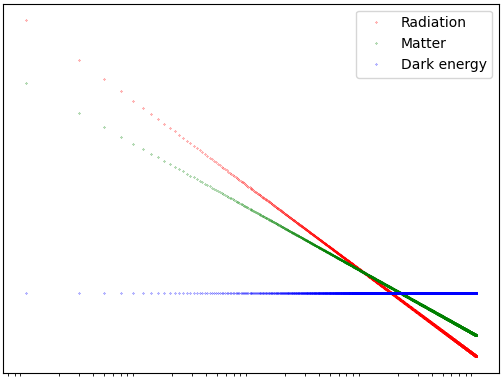
\includegraphics[scale=0.52]{../Figures/Svgs/den.png}
	  \caption{}
	\end{subfigure}
	\caption{(a) Qualitative behaviour of the effective potential in equation (\ref{eq: thy_pot}). Each part the potential \{\textcolor{red}{A}, \textcolor{green}{B}, C\} correponds to different eras dominated by radiation, matter and dark energy respectively. (b) Energy density evolution of radiation, non relativistic matter (dust) and dark energy as contents of the universe (logarithmic scales).}
	\label{Fig: classical_cosmo_pot}
	\end{figure}

Our current observations point to the fact that our universe has entered region $C$ some years ago (around $4\times 10^{9}$ years ago). We can also see that the gradient of this potential in region $C$ is negative, indicating, an accelerated expansion of the universe, in concordance with observations. It is also important to notice the divergence of the potential $V(a)$ when $a \rightarrow 0$, causing a singularity at $t=0$ (conventionally chosen \cite{hawking1970singularities}). What does this mean? From a classical cosmology point of view, this correponds to the \textit{Big bang}\footnote{A given pejorative calificative by those who opposed the proposal that the universe had been in a state with extremely high density, temperature and ridiculous size.}. A singular state that we \textbf{cannot understand} given the tools at hand (i.e general relativity and classical cosmology) where all content of the universe was compacted to a single point at extremely high temperatures \cite{lemaitre1950primeval}. This should already make us bat an eye. We are trying to apply a \textit{classical} framework to a system whose energy regime very well requires a \textit{quantum} description of all the involved forces. It should not then be a surprise that we arrive to singularities in our description if \textit{we are using a sledgehammer to crack a nut}.

But we cannot be so conformist. If we cannot understand through the lenses of a theory as GR, that may be pointing to the fact that our toolbox lacks some important tools. Before we go to our favorite DIY store to buy those tools, we first need to understand \textit{what} and \textit{how} we want to fix our lack of understanding.

We will describe some of the most fundamental flaws of $\Lambda-CDM$ model in the rest of this notes. Solutions can be found in some of the subsequent notes of this collection.

\section*{What is wrong with the $\Lambda$-CDM model?}


\subsection*{The Hubble tension}

The Hubble constant today $H_{0}$, which is determined as the ratio between the velocity and the distance to an object in space ($H_{0} = v/d$), can be measured in two different fashions:

\begin{itemize}
	\item One can obtain the velocity of the object (usually a galaxy) by looking at its redshift. For the distance, the most reliable way is to make use of \textit{standard candles}; Type Ia supernovae whose peak luminosity is the same, no matter where they are in the universe. Given the relation between relative and absolute magnitudes $(m, M)$, it is possible to extract the distance to these objects with good accuracy. This method is used to study "close" celestial objects, i.e. not looking back much into the past. The current value for $H_{0}$ using this method is $H_{0} = 72.3 \pm 1.3 \: km \:s^{-1} Mpc^{-1}$ \cite{2020planck}.
	
	\item An alternative way to obtain $H_{0}$ from observations with our current technology is by studying the CMB, i.e. looking far away in the past. Theoretical predictions for CMB can be obtained by tuning specific parameters in the $\Lambda- CDM$ model, such as curvature, energy densities, etc. One can then compare these predicitions to the observations, to decide which one fits best. The best fiting so far yields a $H_{0}$ value as $67.4 \pm 0.5 \: km \:s^{-1} Mpc^{-1}$ \cite{Riess_2021}
\end{itemize}

As we can see, there is an apparent tension between these two results that technological development has confirmed over the years\footnote{It could have been that our technological limitations were the reason of the difference, but as technology has developed, this difference has been confirmed with better and more realiable measurements.}. What can the reason be to get two different values on the universe expansion rate at two different eras? Several proposals have been debated, without observational confirmation nor agreement in the community yet (see \cite{di2021realm}). In any case, observations point to an existing difference that the standard model cannot (yet) explain.

\subsection*{The cosmological constant problem}

We have talked about different observed values for the same quantity using two different measurement methods. And this is not the only dichotomy which is present in $\Lambda-CDM$.

Let us quantise matter fields appearing in the Einstein-Hilbert action (\ref{eq: EH_action}) as proposed by Weinberg \cite{weinberg1989cosmological}. At the end of the day, the remaining physical interactions (electromagnetism, weak and strong nuclear forces) are quantised in the standard model of particle physics. Each of these interactions, have a \textit{vacuum energy}, which corresponds to the minimum background energy that space itself has. In the absence of curved spacetime, this vacuum energy can be somehow ignored. But, it is not the case when want to study any of these fields in the presence of gravity. By the equivalence principle, we know that gravity couples to all possible forms of energy, and also that of the vacuum.

The quantisation of matter fields will result in an extra constant energy density contribution\footnote{ This extra contribution comes from the closed-loop Feynmann diagrams (i.e. quantum fluctuations around the vacuum state) of each of the matter fields involved. We will not include a discussion of this computation in these notes, but we refer the reader to \cite{Martin_2012, padilla2015lectures} for further reading and details.} to the energy momentum tensor $T_{\mu\nu}$. As this term is constant and with same dimensionality as the cosmological constant (i.e. $[L]^{-2}$), we can add it to $\Lambda$ to obtain an \textit{effective cosmological constant} as:

\begin{equation}
	\Lambda_{\text{eff}} = \Lambda + \underbrace{\kappa^{2}_{4} \rho_{\text{vac}}}_{\Lambda_{\text{vac}}},
\end{equation}

which is in fact the cosmological constant that we are able to measure from observations. Let us now numerically identify each of its contributions. According to \cite{2020planck}, the effective value of the cosmological constant is:

\begin{equation}\label{eq: lambda_eff}
	\Lambda_{\text{eff}} \sim 3 \times 10^{-122} m^{2}_{Pl},
\end{equation}

while any first order correction due to quantum fluctuations of the matter fields is:

\begin{equation}\label{eq: lambda_vac}
	\Lambda_{\text{vac}} \sim \frac{m^{2}_{Pl}}{16 \pi^{2}} \sim 6.3 \times 10^{-3} m^{2}_{Pl}.
\end{equation}

This is about $10^{120}$ order of magnitude of difference (in Planck units), as often stated in the literature. However, previous computations of the vacuum energy are slightly hand-wavy, as the renormalisation scheme does not respect Lorentz invariant. As stated in \cite{Martin_2012}, an accurate renormalisation will return a mismatch of 54 orders of magnitude instead of 120. In both cases, it means that the bare cosmological constant $\Lambda$ has to be extremely fine tuned to cancel in such an almost perfect way to leave the small effective one we can observe. This ultimate required coincidence is what gives title to this section. 

\subsection*{A lack of casual contact}

To understand this final fundamental issue that the standard model of cosmology cannot explain, we first need to define what to be in \textit{contact}\footnote{Awesome cinematographic piece. Highly recommended to watch.} is.

There is nothing faster than light in the universe \cite{carroll2019spacetime}. This imposes an upper bound on the size of a region where two points could have been in casual contact, i.e. information between the points could have travelled in a period of time less or equal than light would have taken to travel the distance that separates them. This region is called the \textit{light cone}.
\vspace{0.5cm} % So the figure can breath!
\begin{figure}[h]
    \centering
    \includesvg[scale=0.4]{../Figures/Svgs/light_cone.svg}
	%Observe that I wrote .. to go the upper directory and navigate to the folder where I have the svg's for all my files.
	\caption{Light cone. Photons travel along world lines of zero proper time, $ds^{2} = 0$, called null geodesics (both lines at $45$ degrees). The set of all null geodesics passing through a given event P in spacetime is called the \textit{light cone}. The interior of the light cone is defined as the region of spacetime causally related to that event P. Casually disconnected events (like Q) are outside the lightcone related to the event P.}
	\label{Fig: light_cone}
\end{figure}

For simplicity in further computations, it is better to describe the propagation of light using the \textit{conformal} time, as:

\begin{equation}
	\eta = \int \frac{dt}{a(t)}.
\end{equation}

Massless particles, as photons, follow null geodesic trajectories, which imply $ds^{2} = 0$. On top of that, as the universe is isotropic, only the radial coordinate will be relevant for computations. This leaves us with:

\begin{equation}\label{eq: distance}
	ds^{2} = a^{2}(\eta)\left[-d\eta^{2} + d\chi^{2}\right]=0 \longrightarrow \chi(\eta) = \eta_{f} - \eta_{i} = \int^{t_{f}}_{t_{i}} \frac{dt}{a(t)},
\end{equation}

where $\chi$ is a generic radial coordinate accounting for all possible topologies \cite{baumann2009tasi}. When $\eta_{i} =0$, $\chi(\eta)$ represents the \textit{comoving particle horizon}, which is the maximum distance light can travel between time 0 and some other time $t$. One can then further rewrite expression (\ref{eq: distance}) in terms of the \textit{comoving Hubble radius} $R_{H} = (a H)^{-1}$, which is the radius of the observable universe at some moment $t$. Then:

\begin{equation}
	\eta_{f} = \int^{t_{f}}_{0} \frac{dt}{a(t)} = \int^{a}_{0} \frac{da}{H a^{2}} = \int^{a}_{0} d \ln(a) \frac{1}{a H}.
\end{equation}

As always, we would like to make contact with today's data, so we can rephrase the Hubble radius at any moment to today's by massaging the first Friedmann equation (\ref{eq: Friedmann1}) together with the energy density evolution (\ref{eq: rho_scaling}) to see that:

\begin{equation}\label{eq: hubble_rad}
	R_{H} = R_{H_{0}} \: a ^{1/2(1+ 3 \omega)}.
\end{equation}

It is important to notice here the dependence of the exponent, which depends on the state parameter $\omega$. This leaves us with a dependence of $\eta$ as :

\begin{equation}
	\eta \propto a^{1/2\left(1+3\omega\right)},
\end{equation}

which means that the comoving horizon grows monotonically with time. This implies that some scales that are entering our horizon today were \textbf{outside} the casual contact horizon in the past (The universe was dominated by radiation and matter, as can be seen in (\ref{Fig: classical_cosmo_pot})). This can be observed in the CMB. Its homogeneity points to the fact that the universe was highly homogenous by that time, but we have just seen that these homogenous regions could not have been in casual contact in the past. How is this possible? What key concept are we missing in our interpretations?

\subsection*{Wrinkles after ironing}

Imagine that you are doing laundry. Normally, when you take your clothes out of the washing machine, they are full of wrinkles. Sometimes get even worse after the clothes dry. Then, you patiently iron them down to flat the surface. Now, try to imagine the opposite case; That your clothes were extremely smooth and flat when you take them out from the washing machine and after you iron, they are still smooth, but not as nicely wrinkleless as they were just when you opened the washing machine door. Makes no sense, Does it? A similar feature is what our universe shows now and then.

Let us rewrite the first Friedmann equation (\ref{eq: Friedmann1}) as:

\begin{equation}\label{eq: divergence_Friedmann}
	\left(\Omega(a)^{-1} - 1\right) \sum \rho_{i} \: a^{2} = -\frac{3k}{8 \pi G_{4}},
\end{equation}

where $\Omega(a) = \sum \rho_{0_{i}} a^{-3(1+\omega)}/\rho_{\text{crit}}$, with $\rho_{\text{crit}} = 3 H^{2}/(8 \pi G_{4})$. Observe that the RHS of previous expression is a constant quantity\footnote{In fact, 0, if we account that $\Omega_{k} \simeq 0$ as we saw in table(\ref{Table: energy_density}).}, while the LHS evolves with time. Density $\rho$ will decrease with time, counterbalanced by the increase of the scale factor $a$. As the universe has been dominated by radiation and matter in the past, this implies that the combination $\rho a^{2}$ has decreased with time. In order to keep the constant behaviour, this requires $\Omega(a)^{-1} -1$ to have increased in the same manner. This constrains further and further the value of $\Omega(a) \simeq 1$ if go back in time. This points to an extreme \textit{fine-tuning} of $\Omega(a)$ at early times, to deviations from one no greater than $\mathcal{O}(10^{-16})$ during the nucleosinthesis period, for example. Any deviation greater than such ridiculously small values would have not granted the flat universe that we observe today.
\vspace{1cm}

With these issues, we finish this \textit{classical cosmology} notes. Although the $\Lambda-CDM$ model has proved its potential to give accurated predictions, confirmed by observations, we have just also seen that it has its flaws and limitations. Solutions to these will be offered in subsequent notes of this series.






\bibliography{biblio}
\bibliographystyle{JHEP}


\end{document}